%-------------------------------------------------------------------------------

\section{Esercizio 1: Convoluzione e sistemi LTI}
La convoluzione tra due segnali è equivalente al loro prodotto nel dominio 
della frequenza. Possiamo riscrivere la funzione di convoluzione dell'esercizio
precedente sfruttando questa relazione matematica:

\begin{equation}
	z(n) = x(n) \circledast y(n) \rightarrow 
	z(n) = F^{-1}(F[x(n)](f) \cdot F[y(n)](f))	
\end{equation}

%-------------------------------------------------------------------------------

\section{Implementazione DFT}
In MATLAB è possibile implementare le DFT e le IDFT come segue:

		
\begin{equation}
	x_{out}[k] = \begin{cases} 
	
	\frac{1}{N} \sum^{N-1}_{n=0} x_{in}[n] 
	e^{j 2 \pi k n / N } & k=0,...,N-1 \\ 
	
	\sum^{N-1}_{n=0} x_{in}[n] 
	e^{- j 2 \pi k n / N } & k=0,...,N-1 
	
	\end{cases}
\end{equation}

dove N è la lunghezza del segnale $x_{in}[n]$.

%-------------------------------------------------------------------------------

\begin{minipage}[t]{.45\textwidth}
	\begin{figure}[H]
	\centering
	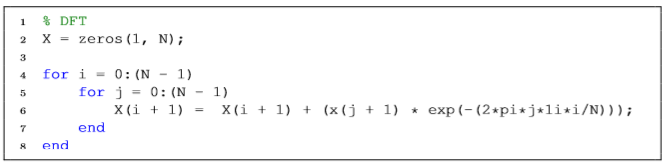
\includegraphics[width=\textwidth]{./images/cap3/DFT.png}
	\caption{Implementazione DFT.}
\end{figure}
\end{minipage}
\hfill
\begin{minipage}[t]{.45\textwidth}
	\begin{figure}[H]
	\centering
	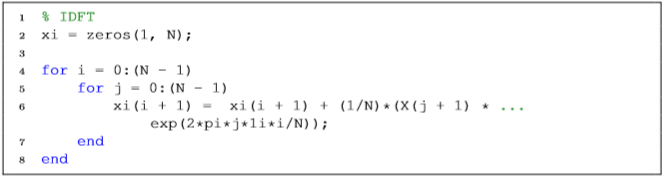
\includegraphics[width=\textwidth]{./images/cap3/IDFT.png}
	\caption{Implementazione IDFT.}
\end{figure}	
\end{minipage}

Le funzioni implementate in questo modo risultano essere equivalenti alle 
funzioni di libreria \textit{fft()} e \textit{ifft()} implementate in MATLAB, 
come si vede in figura \ref{fig:output_L2E2}.

\begin{figure}[H]
\centering
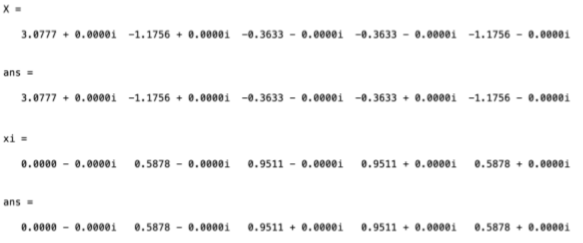
\includegraphics[width=.75\textwidth]{./images/cap3/output_L2E2.png}
\caption{Implementazione MATLAB DFT.}
\label{fig:output_L2E2}
\end{figure}

\section{DFT di segnali analogici}
A partire da un segnale nel tempo $x(t)$ è possibile simularne una versione 
campionata nell’intervallo frequenza di campionamento:

\begin{equation}
	f_c = \frac{1}{T_0}
\end{equation}

nel seguente modo:

\begin{equation}
	x[n] = x(nT_c)
\end{equation}

dove $N=T_0 f_c$ è il numero di campioni. Si considerano, dunque, i seguenti 
segnali:

\begin{itemize}
	\item $x(t) = sinc^2 (t)$
	\item $x(t) = e^{-4|t|}$
	\item $x(t) = cos(2 \pi t)$
\end{itemize}


